\part{Introduction}

An embedded system is a combination of hardware and software components put together to achieve a specific task. Often, embedded systems are built into a larger device or system and are used to process data generated within the device and to control the behaviour of the system. Embedded devices are a category of tiny devices with physical, computational, and power constraints that are programmed to perform dedicated tasks.

Like most of the automotive industry, Scania employs embedded devices called \textit{Electronic Control Units} (ECUs) in their trucks to supervise and regulate essential subsystems like the engine, transmission, braking, and electrical systems. Each of these subsystems contain several ECUs to gather system data and transmit it to a central communicator where the sensor data is processed, and the system operations are monitored.

Scania currently runs a massive fleet of around 600,000 connected heavy vehicles. The company's truck sales make up 62\% of its global sales and Scania has been adding 60,000 trucks to its fleet annually \cite{scania-report}. This large fleet of rolling vehicles that are connected though the communicators opens up new possibilities. These connected devices continuously monitor the state of the vehicle and this data can be used to accurately and efficiently schedule vehicle maintenance. For example, if a tire change is predicted to be required in 100 km then the driver can plan the route smartly to reach the workshop before the vehicle breaks down. This opportunity can be realized by running smart algorithms on the hardware that is currently available.

Machine learning on embedded devices is becoming increasingly popular due to its ability to provide real-time insight and intelligence to devices. This technology can be used to automate tasks, improve efficiency, and make better decisions. But this technology presents a unique set of challenges due to the limited resources available on these devices. Embedded devices are designed to be power efficient, have limited memory and processing power, and require closely tailored algorithms, making it difficult to use pre-existing machine learning models. Furthermore, embedded devices are often expected to produce real-time results, which further complicates the development process. Despite these challenges, machine learning on embedded devices has potential applications in a variety of areas, such as in the fields of robotics and autonomous vehicles.

One such machine learning application that Scania has been developing in their \textsc{LOBSTR} \cite{lobstr} and \textsc{FAMOUS} \cite{famous} projects is \textit{anomaly and fault detection} on the vehicles. Anomalies in this context are patterns in the data that do not conform to the notion of normal behaviour. There are various machine learning techniques available for predicting anomalous behaviour in trucks based on the sensor data readings. The running anomaly detection models for fault prediction on the existing ECUs with limited resources has many benefits and challenges.

\subsection*{Benefits to performing Anomaly Detection on ECUs}

\begin{itemize}
	\item Scania is committed to promote a shift towards autonomous and eco-friendly transport systems. The latest addition of Scania's connected trucks and buses will be embedded with upgraded ECUs and communication devices. However, this upgrade will make the stock of older hardware devices to become obsolete and regarded as e-waste, which could be prevented. Exploring the possibility of repurposing existing ECUs to run machine learning models aligns with Scania's vision of leading the way towards a sustainable future.
	\item Neural networks are a type of machine learning technique that can learn intricate patterns across multiple data signals and time. Neural networks can learn from unstructured data and apply this understanding to unseen data points. Anomaly detection using neural network has the advantage of requiring less manual work in labelling data and can provide paradigms allowing for automation of discovering new and important data points.
	\item Federated learning techniques allow for the ECUs installed in Scania's distributed fleet of connected trucks to perform distributed training leveraging their computational capabilities. Each ECU individually trains the model with its own data and transmits the updated model parameters to a central server. This distributed learning approach enables early detection of faults or failures, reduces the network bandwidth consumption by reducing the sensor data transmission, and ensures that critical data remains on the device.
\end{itemize}

\subsection*{Challenges to implementing Federated Learning on ECUs}

\begin{itemize}
	\item Neural network training is computationally demanding and achieving good performance on embedded devices require careful resource management.
	\item The full potential of implementing neural networks application on embedded devices has still not been realized. Approaches such as TensorFlow Lite, Edge Impulse, and STM Cube AI implemented along with other TinyML frameworks, enable running machine learning models targeted for small resource devices. However, for the neural network models, these approaches are largely limited to inference capabilities. Approaches such as the Tiny Training Engine could potentially unlock the path to training neural network models on embedded devices.
	\item The primary development of the Scania ECU was not completed in house. The information available to Scania regarding aspects of the hardware design is restricted. To construct an embedded operating system for a customized hardware, critical details such as the device tree, memory organization, and boot flow are necessary. Obtaining this information from a functional board can be a difficult task requiring reverse engineering expertise.
\end{itemize}

\subsubsection{Problem Description}

% TODO : Restate the purpose to match the contents of Results / Discussion

The scope of the thesis is to repurpose the existing Scania ECU and explore the challenges of building targeted neural network models and training them on repurposed ECUs using different approaches and evaluating their performances.

\subsubsection{Report Structure}

This report is divided into three parts with multiple chapters containing several sections. The first part describes the background and introduces important information motivating the challenges in performing machine learning on embedded devices. The second part details the benchmark applications that were implemented to evaluate the processes of training neural networks on a specific target device. Lastly, the final part presents an analysis and discussion on implementing the training of a neural network.

% ============================================
%        Background
% ============================================

\chapter{Background}

Developing and maintaining applications that rely on neural network models and run on a fleet of embedded devices has several considerations. The application deployment process should allow for continuous updates to the neural network, transfer data or model updates from the embedded devices to off-board analytics or machine learning pipelines, not interfere with the other applications on the embedded device, all the while maintaining correct representations in the neural network model. It is thus important to have an operating system that can support these applications with features such as process isolation, inter-process communication mechanisms, multitasking etc.

The embedded device that is meant to run the neural network applications are the ECUs aboard a Scania vehicle. These ECUs have ARM application processor cores that are capable of running rich operating systems such as Linux distributions or real-time operating systems such as QNX, or VxWorks. All these operating systems also support hypervisors which allows for configurations where a host operating system runs standard automotive applications in addition to a guest operating system running the neural network application. This approach has the advantage of mitigating application crashes in the guest operating system and can provide a level of protection against software vulnerabilities \cite{Linux-guest-os}. The benchmark applications of interest in this report focuses on training neural network models on environments that use the Embedded Linux operating system.

This chapter introduces several terms and techniques associated with embedded application development and starts with a small section on ARM based embedded boards and hardware connection interfaces. The next section gives an overview of the terminologies and processes associated with Embedded Linux and application development for Embedded Linux boards. The subsequent section introduces a discussion on neural network application development for embedded devices. The final section on federated learning motivates the efforts to study training of the neural network on embedded devices contrasting further with the conventional model of training neural network models for embedded devices.

\section{Embedded Devices}

Embedded systems perform a varied mixture of applications including industrial automation, consumer electronics, automotive, etc. They have capabilities ranging from ultra low power wireless data logging to thrust vector control on rocket ships. Depending on the application domain, embedded devices are generally designed in concert with multiple entities. These entities may be industrial companies that are each responsible for a different hardware or software component.

Consider an example of such an arrangement accounted in this paragraph. The semiconductor and software design company ARM produces ARM processors that are used in a significant fraction of embedded devices due to their power efficiency and versatility. \textit{Silicon vendors} such as Atmel, Qualcomm, NXP, Texas Instruments, etc. buy CPU core designs from ARM and create application processors along with a suite of electrical components in an integrated circuit referred to as a \textit{system on a chip} or SoC. Ultimately, a \textit{system maker} would select among these application processors, sensors, and other peripheral devices to design an embedded \textit{board} for a particular application domain. There are different practises that the industry adopts to create embedded devices for different applications and the example presented here is one among several. The embedded devices considered in this project derive from such a process.

The configuration and functionality of peripheral devices and how they can interact with the processor on the SoC are decided by the silicon vendor. There are several architectural factors that go into this decision such as the computer organization, memory addressing model, supported instruction set architectures, etc. These decision in turn necessitates controller circuits such as for memory access, interrupt control, debug interfaces, etc. Another important component are controllers that enable communication to peripheral devices. These controllers allow communication through standard serial communication buses such as Serial Peripheral Interface (SPI), Inter-Integrated Circuit (I2C), Universal Serial Bus (USB), Universal Asynchronous Receiver-Transmitter (UART), etc. The sum of the decision factors behind how the SoC is organized determine its hardware software interface.

Depending on the application domain, a system maker has to select the right SoC, peripheral devices, and some additional controllers to facilitate communication with those peripherals. These components are then generally laid out on a Printed Circuit Board (PCB) there by creating the embedded board, sometimes also referred to as a System on Module (SoM). The PCB is then enclosed in some casing that also holds sensors or actuators that the embedded system requires. A simplified diagram of an ARM based embedded board is presented in Figure \ref{fig:arm-scheme}

\begin{figure}[h]
	\centering
	\begin{tikzpicture}[font=\small, >=Stealth]

		\fill [fill=orange!30] (0, 0) rectangle (14, 5);
		\draw (7, 5.25) node {Board};

		\fill [fill=yellow!30] (4, 0) rectangle (10, 4.5);
		\draw (7, 4.25) node {System on Chip};

		\draw [fill=cyan!40, draw=cyan] (6, 2) rectangle (8, 4);
		\draw (7, 3) node[align=center, font=\normalsize]
			{ARM \\ Cortex A9};

		\draw [line width=0.42em] (7, 2) -- (7, 0);
		\draw (7.5, 1.5) node[align=center, font=\tiny]
			{Internal \\ SoC bus};

		\draw [fill=green!40, draw=green] (4.25, 1.1) rectangle (5.8, 1.95);
		\draw (5, 1.5) node[align=center] {SPI \\ controller};
		\draw [<-, very thick] (5.8, 1.5) -- (7, 1.5);

		\draw [fill=green!40, draw=green] (4.25, 0.1) rectangle (5.8, 0.95);
		\draw (5, 0.5) node {UART};
		\draw [<-, very thick] (5.8, 0.5) -- (7, 0.5);

		\draw [fill=purple!30, draw=purple] (1.5, 1) rectangle (3, 2);
		\draw (2.25, 1.5) node[align=center] {SPI \\ device};
		\draw [<-, very thick] (3, 1.5) -- (4.25, 1.5);

		\draw [very thick] (3.65, 1.5) -- (3.65, 3);

		\draw [fill=purple!30, draw=purple] (1.5, 2.5) rectangle (3, 3.5);
		\draw (2.25, 3) node[align=center] {SPI \\ device};
		\draw [<-, very thick] (3, 3) -- (3.65, 3);

		\draw [fill=green!40, draw=green] (8.2, 0.6) rectangle (9.75, 1.45);
		\draw (9, 1) node[align=center] {I2C \\ controller};
		\draw [->, very thick] (7, 1) -- (8.2, 1);

		\draw [very thick] (10.4, 1) -- (10.4, 4);

		\draw [fill=purple!30, draw=purple] (11, 0.5) rectangle (12.5, 1.5);
		\draw (11.75, 1) node[align=center] {I2C \\ device};
		\draw [->, very thick] (9.75, 1) -- (11, 1);

		\draw [fill=purple!30, draw=purple] (11, 2) rectangle (12.5, 3);
		\draw (11.75, 2.5) node[align=center] {I2C \\ device};
		\draw [->, very thick] (10.4, 2.5) -- (11, 2.5);

		\draw [fill=purple!30, draw=purple] (11, 3.5) rectangle (12.5, 4.5);
		\draw (11.75, 4) node[align=center] {I2C \\ device};
		\draw [->, very thick] (10.4, 4) -- (11, 4);

	\end{tikzpicture}
	\caption{Simplified schematic view of an ARM Device}
	\label{fig:arm-scheme}
\end{figure}

\subsection{A Brief Overview of ARM Processor Families}

ARM processor cores are ubiquitous in embedded systems and come in 3 primary flavours for their use in embedded devices. The architecture implemented by these different categories of processors also differ in their nature and complexity. The Cortex A series of processors implement the ARM Application profile (A-profile) architecture and are general purpose, high performance cores with capabilities such as virtual memory addressing, support for multiple processing units, secure boot through hardware enforced isolation, and more. The memory management unit present in these cores makes it easier to run modern operating systems on them. These embedded processor cores are primarily used in smartphones, laptops, network appliances, set-top boxes, medical devices, etc. The Cortex R series of processors implement the ARM Real-time profile (R-profile) architecture with its tightly coupled memory and fault tolerance features target real time applications such as solid state device controllers, media players, airbags, braking systems, etc. Cortex R processors do not have memory management units and instead implement a protected memory system architecture due to their requirement to support hard real time applications. A suitable modified Linux can be made to run on Cortex R, however the cores more commonly runs ARM's real time operating system Mbed OS. Lastly, the Cortex M series of processor cores implement ARM Microcontroller profile (M-profile) and are low-cost, energy-efficient cores targeting microcontroller applications. Cortex M cores are notably simpler compared to Cortex A or Cortex R and commonly run bare metal programs as well as Mbed OS.

\begin{table}[h]
	\centering
	\begin{tabular}{ |p{5em}|p{10em}|p{7em}|p{10em}| }
		\hline
			\textbf{SoC} &
			\textbf{Application Domain} &
			\textbf{Architecture} &
			\textbf{Processor Core} \\
		\hline
			nRF51822 &
			Ultra low power, BLE &
			ARM v6-M &
			ARM Cortex M0 \\
		\hline
			AM2732 &
			Automotive &
			ARM v7-R &
			ARM Cortex R5 \\
		\hline
			AM3358 &
			Industrial / IoT &
			ARM v7-A &
			ARM Cortex A8 \\
		\hline
			i.MX6S &
			Multimedia applications &
			ARM v7-A &
			ARM Cortex A9 \\
		\hline
			Kryo 240 &
			Smartphones &
			ARM v8-A &
			ARM Cortex-A73, A53 \\
		\hline
	\end{tabular}
	\caption{A few ARM application processors with their domains, cores, and architecture}
	\label{table:arm}
\end{table}

The popular open source educational single board computer BeagleBone Black (Figure \ref{fig:bbb}) has an ARM Cortex A8 based Texas Instruments AM3359 processor core. Table \ref{table:arm} lists further examples of different ARM based SoCs, their Application Domain, Processor Cores, and specific Architecture Profiles. Embedded Linux is commonly found on Cortex A based processor series such as the one present in the BeagleBone.

\begin{figure}[h]
	\centering
	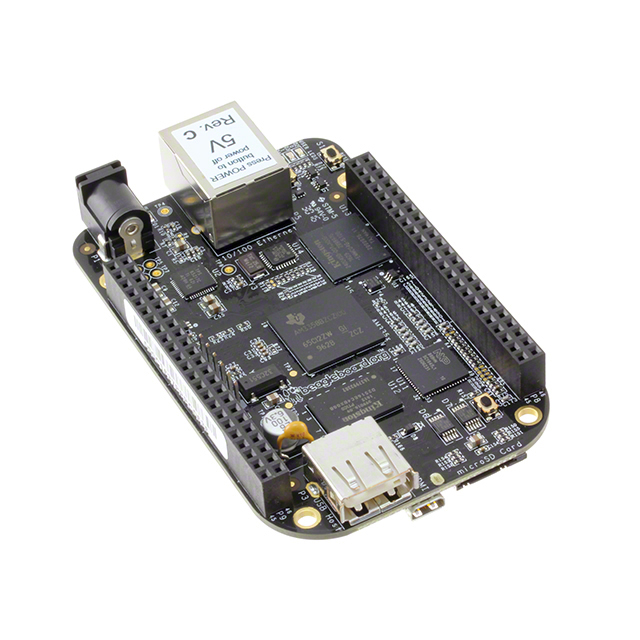
\includegraphics[scale=0.34]{bbb.jpeg}
	\caption{BeagleBone Black}
	\label{fig:bbb}
\end{figure}

\subsection{Hardware Connection Interfaces for Embedded Devices}

Embedded devices rely on a diverse array of hardware connection interfaces to facilitate communicating with other devices, debugging, or for user interaction. These interfaces enable devices to exchange data, configuration settings, and control signals. The connectors play a critical role in the development, testing, and operation of the embedded hardware device. Here, we explore some essential and common hardware connection interfaces for embedded devices.

\subsubsection{General Purpose Input/Output (GPIO) pins}

GPIO pins are versatile and fundamental components of embedded devices. They allow digital signals to be both input and output, enabling devices to interface with the external world. GPIO pins can be used for tasks such as reading sensors, controlling actuators, and communicating with other devices using protocols like I2C or SPI.

SPI and I2C are serial communication protocols that enable devices to exchange data with peripherals such as sensors, displays, and memory. SPI utilizes multiple data lines for high-speed, full-duplex communication. I2C, on the other hand, employs two wires and supports multiple devices on a shared bus. Both protocols offer efficient communication and are well-suited for connecting embedded systems to various external components.

\subsubsection{UART (Universal Asynchronous Receiver-Transmitter)}

UART is a simple and widely adopted asynchronous serial communication interface that facilitates the transmission of data between devices. It employs asynchronous communication, with data being sent as a stream of bits along with start and stop bits. The precise timing of the communication can be controlled by the communication channel such as USB. UART connections are commonly used for console output, firmware updates, and device configuration. They provide a straightforward method for devices to communicate over short distances.

\subsubsection{JTAG (Joint Test Action Group) Debug Ports}

JTAG is a standardized interface used for debugging and testing embedded systems. It allows developers to access and manipulate internal components of a device, including CPUs, memory, and other integrated circuits. JTAG enables operations like boundary scanning, which aids in identifying manufacturing defects, as well as in-circuit debugging to inspect and modify a device's state during runtime. Developer tools meant to configure and test an embedded board usually make heavy use of this interface.

\subsubsection{Ethernet and Wi-Fi}

For network connectivity, embedded devices can integrate Ethernet ports or Wi-Fi modules. Ethernet enables wired communication and is suitable for applications requiring high data rates and low latency. Wi-Fi, on the other hand, provides wireless connectivity, allowing devices to communicate over local or wide area networks. Both options enable embedded devices to connect to the internet, exchange data with remote servers, etc.

There are even more interfaces commonly found within embedded devices such as the USB, or the Controller Area Network (CAN) communication protocol which is commonly used in automotive applications. These hardware connection interfaces are an important part of interfacing with embedded devices. They enable integrations with other sensors and devices, communication with the outside world, and control of the system. Each interface caters to specific use cases, contributing to the versatility and functionality of embedded systems across industries and applications.

The upcoming sections explore the software development process for embedded devices that use the Embedded Linux operating system.

\section{Embedded Linux and Application Development}

Creating application programs and building a particular distribution of an Embedded Linux kernel requires a suite of software programs. This section presents an overview of aspects of this software stack, focusing on the categories of critical tools that facilitate development in the domain of Embedded Linux. Communicating with an embedded system requires hardware specific connectors and matching software tools. Additionally, the concept of the cross compiling toolchain will be explored, highlighting their significance in enabling developers to build software for hardware architectures different from the development machine. After that, the section explores a software system that is used to generate a bootable executable file for an Embedded Linux kernel. The concluding part of the section demonstrate the use of QEMU emulator as a means of embedded application development.

\subsection{Software Development Kits}

Creating applications for embedded devices requires a set of software components that are usually collectively referred to as a \textit{Software Development Kit} (SDK). This suite of programs usually contain a \textit{toolchain} that is capable of converting application source code, such as those in \texttt{C}  or \texttt{C++}, into executables that can be run on an embedded device. A simplified account for that process now follows.

\texttt{C} and \texttt{C++} programming languages are implemented in such a way that source code written in either language has to be first read by a \textit{compiler} program, which will then generate machine code in the form of an \textit{object file}. The primary choice for a \texttt{C} compiler in the embedded domain is the GNU Compiler Collection \texttt{gcc}, with LLVM's \texttt{clang} being a close alternative.

\begin{figure}[H]
	\centering
	\begin{tikzpicture}
		\node [box] (source) {Source Code};
		\node [box, right=of source, fill=red!20] (compiler) {Compiler};
		\node [box, right=of compiler] (objects) {Object files};

		\draw [next] (source) -- (compiler);
		\draw [next] (compiler) -- (objects);
	\end{tikzpicture}
\end{figure}

The object files of a program generated via the compiler together with their required libraries, which are usually themselves object files of some kind, will then be combined by another program referred to as a \textit{linker}. The linker merges the object files taking care to identify their interdependencies to generate another object file, or possible an \textit{executable file}. The GNU project linker program \texttt{ld} is a popular choice used in the embedded domain, while for LLVM project has its own replacement utility called \texttt{LLD}.

\begin{figure}[H]
	\centering
	\begin{tikzpicture}
		\node [box] (objects) {Source Object files};
		\node [box, right=of objects, fill=red!20] (linker) {Linker};
		\node [box, above=of linker] (libraries) {Library Object files};
		\node [box, right=of linker] (executable) {Executable file};

		\draw [next] (objects) -- (linker);
		\draw [next] (libraries) -- (linker);
		\draw [next] (linker) -- (executable);
	\end{tikzpicture}
\end{figure}

Finally, a \textit{loader} program then takes this executable file and places it in memory such that it can begin its execution. A similar program to a compiler is the \textit{assembler} which takes an assembly file as input before generating an object file. Another useful program in this context is the \textit{debugger}, which is a tool used to test a program. Again, the GNU project's debugger is the \texttt{GDB} with the LLVM project alternative being \texttt{LLDB}.

The toolchains used for software development consists of a compiler, linker, libraries, and debuggers. Additionally, the toolchain will have a collection of programs to create and manage executable binary programs. An example for the same is the commonly used GNU binary utilities, a.k.a. binutils. To develop applications that interface with the Linux operating system APIs, a toolchain targeting a Linux operating system will also contain the necessary header files called \textit{Linux kernel header files}. These header files encode the user level Linux API that user-level applications can use to interact with and utilize the different features of the Linux kernel. As an example, System level utility software programs make heavy use of this interface to provide their functionality.

The final important piece of a toolchain will be the \texttt{C} runtime library, which is the primary component that enables the execution of \texttt{C} and \texttt{C++} programs. It provides essential functionality in the form of functions and routines to interact with the operating system, manage memory, and perform various Input Output (I/O) operations. The most popular choice of a \texttt{C} runtime library is GNU's \texttt{glibc}. Alternatives include \texttt{musl libc} and \texttt{uClibc}.

\subsection{Cross Compiling}

The software development toolchains for embedded devices are generally run on a development machine that is different from the embedded device. In this configuration the compiler toolchain creates executables for a different device that the one it is currently running on and is termed a \textit{cross compiling} toolchain. A compiler toolchain that creates executables for the sample device is termed a \textit{native} compiler toolchain. Cross-compilers are common due to several factors such as limited resources on embedded devices, ease of targetting multiple hardware devices, etc. and they are ultimately an unavoidable part of creating programs for a new hardware device. Most software that are run on embedded devices are created on a different computing device. Such a computing device in the context of cross compilation is referred to as a \textit{development host} and the embedded device that the software ultimately runs on is called the \textit{target}.

\begin{figure}[H]
	\centering
	\begin{tikzpicture}
		\node [box] (source) {Source Code};
		\node [box, fill=red!20, above=of source] (cross) {Cross Compiler};
		\node [box, right=of cross] (target) {Target Binaries};

		\begin{scope}[on background layer]
			\fill [violet!15] ([xshift=-7pt, yshift=-7pt]source.south west) rectangle ([xshift=7pt, yshift=7pt]cross.north east);
			\node [yshift=14pt] at (cross.north) {\textbf{Development Host}};

			\fill [purple!15] ([xshift=-7pt, yshift=-7pt]target.south west) rectangle ([xshift=7pt, yshift=7pt]target.north east);
			\node [yshift=14pt] at (target.north) {\textbf{Target Machine}};
		\end{scope}

		\draw [next] (source) -- (cross);
		\draw [next] (cross) -- (target);
	\end{tikzpicture}
\end{figure}

\subsubsection{A short introduction to the ARM GNU toolchain}

A toolchain can usually be described by a quadruple taking the general format \texttt{<arch>}-\texttt{<vendor>}-\texttt{<os>}-\texttt{<libc/abi>}. \texttt{<arch>} stands for the target CPU architecture for the binaries that will be produced by the toolchain, the system manufacturer or vendor who is responsible for the hardware is \texttt{<vendor>}, \texttt{<sys>} generally stands for the operating system or takes the special value \texttt{none} for bare-metal, and the target application binary interface or \texttt{C} runtime is \texttt{<libc/abi>}. This tradition of naming toolchains exists across build automation tools, compiler projects, etc in different ways under different names such as system definitions in autoconf, or the target triple in LLVM\textquotesingle s Clang. Another naming convention used for the \texttt{<arch>} string when referring to ARM architectures is the use of strings such as \texttt{armv7} to denote the ARMv7 architecture found in ARM Cortex A (ARMv7-A), ARM Cortex R (ARMv7-R), and ARM Cortex M (ARMv7-M) cores.

ARM GNU toolchain is a GNU toolchain for ARM architecture that is released and maintained by ARM and from open-source project GCC, Binutils, glibc, Newlib, and GDB. The toolchain supports \texttt{C} and \texttt{C++} languages and supports CPUs based on the A, R, and M profiles of the ARM architectures.

\subsection{Embedded Linux Build Systems}

Building and maintaining Embedded Linux distributions with the Linux kernel and user mode applications require tools that can support multi-level build configurations, interface with or build a cross compiling toolchain, support \texttt{C} run times such as \textit{glibc} or \textit{musl} libc, and provide support for project management. There are several tools that provide this support such as OpenADK, The Yocto Project, Buildroot, OpenWrt, etc., with The Yocto Project and Buildroot being the most feature full and widely used Embedded Linux build systems. In comparison with Buildroot, the Yocto Project supports a greater variety of hardware and also has faster incremental build times as it caches the generated binaries \cite{yocto} making it ideal for managing Embedded Linux builds for diverse hardware devices. The Yocto Project with its ability to create tailored and optimized Linux distributions, its comprehensive toolset, and its focus on reproducibility and flexibility was chosen as the primary build system for this project and was used to generate the associated Embedded Linux and application programs.

Building an Embedded Linux kernel suited for a mainboard of an embedded device requires appropriate build configurations describing the kernel, its enabled feature, the device tree layout, i/o memory mapping, etc \cite{bootlin-port}. These parameters are a description of the devices on the mainboard, their interfaces to the processor, and the nature of the Embedded Linux that is to be managing the hardware device. The collection of software and configurations required to get an operating system running on a board is referred to as a \textit{Board Support Package} (BSP).

\begin{figure}
	\centering
	\begin{tikzpicture}
		\node [fill=cyan!20, draw=cyan, bigbox] (upstream) at (0, 0) {};
		\node [align=center, font=\large] at ([yshift=-2em]upstream.north) {Upstream \\ Project};
		\node [align=center, font=\small] at ([yshift=2em]upstream.south) {Official version \\ Open Source};
		\node [fill=yellow!20, draw=yellow, bigbox] (vendor) at ([xshift=7em]upstream.east){};
		\draw [-{Latex}, very thick] (upstream.east) -- (vendor.west);
		\node [align=center, font=\large] at ([yshift=-2em]vendor.north) {SoC vendor \\ fork};
		\node [align=center, font=\small] at ([yshift=2em]vendor.south) {Suppports SoC vendor \\ evaluation boards};
		\node [fill=red!20, draw=red, bigbox] (system) at ([xshift=7em]vendor.east){};
		\draw [-{Latex}, very thick] (vendor.east) -- (system.west);
		\node [align=center, font=\large] at ([yshift=-2em]system.north) {Board/SoM \\ fork};
		\node [align=center, font=\small] at ([yshift=2em]system.south) {Supports board/SoM};
	\end{tikzpicture}
	\caption{Software Sourcing for a Board Support Package}
	\label{fig:software-versions}
\end{figure}

The process of sourcing software packages for a BSP involves several components, outlined in Figure \ref{fig:software-versions}. At the core of this process lies the \textit{Upstream Project}, which represents the official and open-source version of software components. An example of an upstream project would be the Linux source code. The upstream version is maintained by the broader community and serves as the foundation for various platforms. The development practises surrounding upstream projects are generally within the open source ethos.

As the software moves downstream, it encounters forks created by SoC vendors. These \textit{SoC vendor forks} are tailored to support specific boards produced by the SoC vendors. The classic example would be of the \textit{evaluation board}. An evaluation board in this context is a hardware platform specifically designed by SoC vendors or other technology companies to showcase and evaluate the features and capabilities of a particular SoC. While the SoC vendor forks facilitate hardware-specific optimizations, they may lean more toward proprietary code and thus have a reduced level of openness compared to the upstream version.

The subsequent downstream layer is of a \textit{Board/SoM fork}, where the software is adapted to cater to the intricacies of particular boards or System on Module. The fork is required to target the particular board as neither the upstream project, nor a SoC vendor fork may be easily used to get the necessary binaries to target the board. This layer introduces another level of customization and specialization but can also vary in terms of openness. In some cases, these forks might be proprietary or closely guarded, contributing to a degree of fragmentation within the embedded ecosystem. This fragmentation arises as different board and SoM makers create their own customized versions, potentially hindering interoperability and collaborative development efforts.

In essence, the movement of software from upstream to downstream involves a trade-off between customization and openness. While customization is crucial for optimizing software to run efficiently on specific hardware, it's essential to strike a balance that promotes openness and collaboration. Overreliance on close-source forks can lead to ecosystem fragmentation, making it challenging to leverage the collective wisdom and expertise of the broader open-source community.

\subsubsection{The Target Embedded Device}

To port Linux onto a processor on a particular board requires creating a \textit{bootloader} program capable of that task as well. A bootloader is responsible for placing an operating system into memory and handing over the control of the processor. The technical details as to how the bootloader has to be configured will be based on the particulars of the hardware that it will be configured for.

The initial target machine for the project was an ECU playing the role of a communicator on the truck. The BSP source code for the board however was unavailable as well as certain critical support components for the board, such as the system maker's Yocto meta layer, memory mapping for the attached devices, source codes for boot ROM firmware or the bootloader, etc. The reverse engineering efforts to attain this information were dropped due to time constraints, the details of the attempt to uncover this information is laid out in Appendix \hyperref[rtc-c300]{I}. Ultimately, the MCIMX6Q-SDB evaluation board (Figure \ref{fig:mcimx6q-sdb}) was chosen as an alternative to the ECU. The required information for the MCIMX6Q-SDB is publicly provided by processor chip vendor NXP.

\subsubsection{A brief aside on Continuous Integration and Continuous Delivery}

An important aspect for software development in general are the ideas behind Continuous Integration (CI) and Continuous Delivery (CD). CI/CD are modern software development practices that focus on automating and streamlining the process of building, testing, and deploying software. CI is the practise of frequently integrating code changes into a shared repository, performing automated tests to identify and fix issues that arise from such integration efforts, and promoting collaboration, early bug detection, and code quality improvements. CD extends the ideas in CI by automating the deployment of code to production environments. It enables rapid, reliable, and consistent software releases and aims to deliver code changes to end users quickly and efficiently. CI/CD practises foster a culture of automation and agility, allowing development teams to deliver high-quality software more frequently and with greater confidence. CI/CD has been quickly adopted to modern software development practises including embedded software development.

\begin{figure}[h]
	\centering
	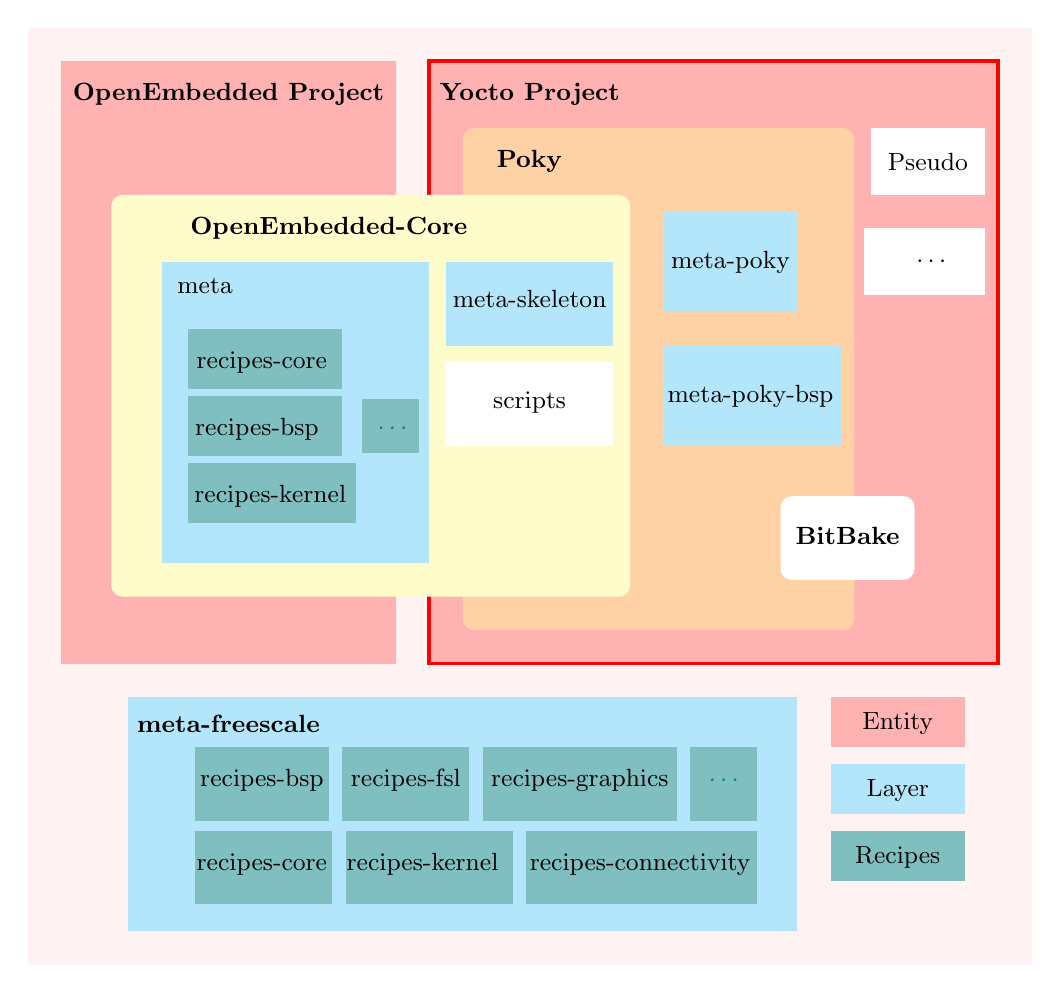
\begin{tikzpicture}[font=\small, scale=0.85]

		\fill [fill=pink!20] (-0.5, -4.5) rectangle (14.5, 9.5);

		\fill [fill=red!30] (0, 0) rectangle (5, 9);
		\draw (2.5, 8.5) node {\textbf{OpenEmbedded Project}};

		\draw [fill=red!30, draw=red, line width=1.4pt] (5.5, 0) rectangle (14, 9);
		\draw (7, 8.5) node {\textbf{Yocto Project}};

		\fill [orange!35, rounded corners] (6, 0.5) rectangle (11.85, 8);
		\draw (7, 7.5) node {\textbf{Poky}};

		\fill [yellow!20, rounded corners] (0.75, 1) rectangle (8.5, 7);
		\draw (4, 6.5) node {\textbf{OpenEmbedded-Core}};

		\fill [cyan!30] (1.5, 1.5) rectangle (5.5, 6);
		\draw (2.15, 5.65) node {meta};

		\fill [teal!50] (1.9, 4.1) rectangle (4.2, 5);
		\draw (3, 4.5) node {recipes-core};

		\fill [teal!50] (1.9, 3.1) rectangle (4.2, 4);
		\draw (2.925, 3.5) node {recipes-bsp};

		\fill [teal!50] (1.9, 2.1) rectangle (4.4, 3);
		\draw (3.125, 2.5) node {recipes-kernel};

		\fill [teal!50] (4.5, 3.15) rectangle (5.35, 3.95);
		\draw (4.95, 3.5) node[text=teal] {\textbf{$\cdots$}};

		\fill [cyan!30] (5.75, 4.75) rectangle (8.25, 6);
		\draw (7, 5.45) node {meta-skeleton};

		\fill [white!40] (5.75, 3.25) rectangle (8.25, 4.5);
		\draw (7, 3.9) node {scripts};

		\fill [cyan!30] (9, 5.25) rectangle (11, 6.75);
		\draw (10, 6) node {meta-poky};

		\fill [cyan!30] (9, 3.25) rectangle (11.65, 4.75);
		\draw (10.3, 4) node {meta-poky-bsp};

		\fill [white!40, rounded corners] (10.75, 1.25) rectangle (12.75, 2.5);
		\draw (11.75, 1.9) node {\textbf{BitBake}};

		\fill [white!40] (12.1, 7) rectangle (13.8, 8);
		\draw (12.95, 7.5) node {Pseudo};

		\fill [white!40] (12, 5.5) rectangle (13.8, 6.5);
		\draw (13, 6) node {\textbf{$\cdots$}};

		\fill [cyan!30] (1, -4) rectangle (11, -0.5);
		\draw (2.5, -0.9) node {\textbf{meta-freescale}};

		\fill [teal!50] (2, -2.35) rectangle (4, -1.25);
		\draw (3, -1.75) node {recipes-bsp};

		\fill [teal!50] (4.2, -2.35) rectangle (6.1, -1.25);
		\draw (5.15, -1.75) node {recipes-fsl};

		\fill [teal!50] (6.3, -2.35) rectangle (9.2, -1.25);
		\draw (7.75, -1.75) node {recipes-graphics};

		\fill [teal!50] (9.4, -2.35) rectangle (10.4, -1.25);
		\draw (9.9, -1.75) node[text=teal] {\textbf{$\cdots$}};

		\fill [teal!50] (2, -3.6) rectangle (4.05, -2.5);
		\draw (3, -3) node {recipes-core};

		\fill [teal!50] (4.25, -3.6) rectangle (6.75, -2.5);
		\draw (5.4, -3) node {recipes-kernel};

		\fill [teal!50] (6.95, -3.6) rectangle (10.4, -2.5);
		\draw (8.65, -3) node {recipes-connectivity};

		\fill [red!30] (11.5, -1.25) rectangle (13.5, -0.5);
		\draw (12.5, -0.9) node {Entity};

		\fill [cyan!30] (11.5, -2.25) rectangle (13.5, -1.5);
		\draw (12.5, -1.9) node {Layer};

		\fill [teal!50] (11.5, -3.25) rectangle (13.5, -2.5);
		\draw (12.5, -2.9) node {Recipes};
	\end{tikzpicture}
	\caption{Overview of The Yocto Project Components}
	\label{fig:yocto-overview}
\end{figure}

\subsubsection{An overview of the Yocto Project Embedded Linux build system}

Embedded Linux build systems can become fairly large and complicated software stacks depending on their supported development scenarios, the number and the nature of Software Engineers using the tool, the CI/CD infrastructure, and the list of supported hardware devices.

The Yocto Project is arranged into several components out of which the core 3 components are BitBake, OpenEmbedded-Core, and Poky. BitBake is a build engine that interprets configuration files to schedule and then perform tasks. The configuration files, also called  \textit{recipes}, describe how to build a particular package such as a shared library or application program. Recipes contain information as to where to obtain the source code for a package, instructions for compiling the source code, and installing or removing that package from a distribution. OpenEmbedded-Core is a set of device and distribution independent recipes and other metadata. Poky is a reference system containing a collection of projects and tools that can be used to bootstrap a new distribution.

The Yocto Project emerged from the development of the OpenEmbedded build automation framework and jointly maintains core components of the OpenEmbedded build system. The OpenEmbedded Core originated from a separation of recipe metadata within OpenEmbedded.  The Yocto Project's overall structure can appear intricate, with a multitude of terms and techniques contributing to its steep learning curve. A simplified representation of the Yocto Project is shown in Figure \ref{fig:yocto-overview}. It depicts sets of recipes (teal) grouped into a \textit{layer} (cyan). Layers can have dependencies on other layers. Multiple layers are often used in a single Embedded Linux distribution. Note that a legend is also present in the bottom right of the diagram in Figure \ref{fig:yocto-overview}.

\begin{figure}[h]
	\centering
	\begin{tikzpicture}[font=\small, >=Latex]

		\fill [fill=pink!20] (0, 0) rectangle (11, 7.5);

		\fill [fill=blue!30] (0.5, 3.5) rectangle (4.5, 6);
		\draw (2.5, 6.21) node {\textbf{Yocto Project Machine}};
		\draw (2.5, 4.75) node[align=left]
			{
				Hosts Yocto Project \\
				Can Host an SDK \\
				Can Build an SDK \\
				Can Build an Image \\
				Can Build an Application
			};

		\draw [<-, very thick] (4.5, 5.2) -- (7.5, 5.2);
		\draw (6, 5.4) node {Objects};

		\fill [fill=green!30] (7.5, 4.7) rectangle (10.5, 6.5);
		\draw (9, 6.7) node {\textbf{Development Machine}};
		\draw (9, 5.6) node[align=left]
			{
				Compile Code \\
				Debug Code \\
				Hosts an SDK
			};

		\draw [<-, very thick] (4.5, 3.75) -- (7.5, 3.75);
		\draw (6, 3.95) node {Objects};

		\fill [fill=green!30] (7.5, 2.3) rectangle (10.5, 4.1);
		\draw (9, 4.3) node {\textbf{Development Machine}};
		\draw (9, 3.2) node[align=left]
			{
				Compile Code \\
				Debug Code \\
				Hosts an SDK
			};

		\draw [->, line width=0.42em] (2.5, 3.5) -- (2.5, 2.2);
		\draw (3.4, 3.1) node {Deploy};

		\fill [fill=red!30] (1, 0.5) rectangle (5, 1.75);
		\draw (2.5, 2) node {\textbf{Target Hardware}};
		\draw (3, 1) node[align=left]
		{
			Boots and Runs Images \\
			Runs Applications
		};

	\end{tikzpicture}
	\caption{Simplified overview of an Application development practise using the Yocto Project}
	\label{fig:yocto-dev}
\end{figure}

The Yocto Project can be used work on several aspects of Application and Kernel level development for Embedded Linux. Application development in the Yocto Project can be thought to have several practises such as arranging the information regarding the application packaging in a related metadata layer within BitBake recipes. The development process would also have multiple computer machines associated with it as shown in the diagram in Figure \ref{fig:yocto-dev}. In this model, the Yocto Project machine is the core environment for building the software stack, including the Linux kernel and user space applications. The development machine is used for coding, compiling, and debugging applications, while an embedded device runs the final images and executes the developed applications. Appendix \hyperref[yocto-setup]{II} showcases an example usage of the Yocto Project.

\subsection{Application development using QEMU}

Another common alternative to cross compiling in this manner is by using native compilers via emulation. Emulation is some technique that allows a \textit{host} computer system to simulate the behaviour of some other \textit{guest} computer system. There are several software projects that allow for emulation in this manner with QEMU being by far the most commonly used emulator targetting different hardware devices. QEMU can also be used to create and test embedded applications before being deployed on the target hardware. Application development for embedded devices usually employs a combination of cross compiling toolchains and emulation software to create, test, and maintain the software.

\subsubsection{An example Embedded Development Environment on Linux using QEMU}

In this section let's consider a simple development environment capable of compiling and executing \texttt{C} programs for an \texttt{armv7} ARM processor using a personal computer running Linux. This setup leverages features of the Linux operating system running on the development host and the capabilities of the QEMU machine emulation system. The code listings in this section were tested on a fedora workstation operating system. As with the previous code listings within the section about the Yocto Project, some commands may break their interfaces, such as fedora\textquotesingle s package manager utility \texttt{dnf}. However, the general principles maybe used to create a similar setup on Linux distributions.

The Linux kernel has a feature called \texttt{binfmt\_misc} which stands for \textit{Miscellaneous Binary Format}. This feature allows for interpreter programs to be associated and invoked upon using certain binary format files. Together with the \texttt{chroot} command, \texttt{binfmt\_misc} can be leveraged to set up an environment that can use a QEMU emulator program to test and develop for a different architecture than that of the development host.

The interpreter programs registered with \texttt{binfmt\_misc} are usually user space applications such as emulators and virtual machines. For this section the interpreter program will be a QEMU user space emulator program, namely \texttt{qemu-arm}. QEMU has multiple operating modes apart from a full system emulation such as its user-mode emulation mode. In user-mode emulation, QEMU can perform system call translation and POSIX signal handling in Linux which effectively allows for programs compiled for a different instruction set to be executed using QEMU. Cross compiling and cross debugging are common use cases for this user-mode emulation in QEMU. \texttt{qemu-arm} is a QEMU User space emulator program for executing programs compiled for ARM.

After an interpreter and binary file format pair are registered, \texttt{binfmt\_misc} recognizes the associated binary files by matching some bytes at the beginning of a file with a magic byte sequence that had been supplied. The usage of magic bytes at the beginning of files is a UNIX tradition adopted as a means of incorporating file type metadata within the file.

As with some Linux features, \texttt{binfmt\_misc} must first be mounted at specific location after which it can be configured. If \texttt{binfmt\_misc} is not already present at the default path location at \texttt{/proc/sys/fs/binfmt\_misc}, it may be mounted by using the following command.

\begin{minted}{bash}
mount binfmt_misc -t binfmt_misc /proc/sys/fs/binfmt_misc
\end{minted}

To register the binary format and interpreter pair to set up the development environment, a string of the form \texttt{:name:type:offset:magic:mask:interpreter:flags} needs to be sent (\texttt{echo}ed) to the \texttt{register} file at the path mentioned previously. Assuming that \texttt{qemu-arm} is present at the path \texttt{/usr/bin}, running the following command will register \texttt{qemu-arm}

\begin{minted}{bash}
echo ":qemu-arm:M::\x7fELF\x01\x01\x01\x00\x00\x00" "\x00\x00\x00\x00\x00\x00\x02\x00\x28\x00:" "\xff\xff\xff\xff\xff\xff\xff\x00\xff\xff" "\xff\xff\xff\xff\xff\xff\xfe\xff\xff\xff:" "/usr/bin/qemu-arm-static:F" > /proc/sys/fs/binfmt_misc/register
\end{minted}

Note that the \texttt{echo} should produce a string without whitespaces. A new file named \texttt{qemu-arm} will show up in the path \texttt{/proc/sys/fs/binfmt\_misc/} upon successful completion of the \texttt{echo} command.

Another Linux feature is \texttt{chroot} which allows for changing the apparent root directory of a running process and its children. \texttt{chroot} system call interface started with UNIX and is useful for testing and developing software systems in a modified test environment.

Prior to running \texttt{chroot}, a root directory for the target environment must be prepared. A root directory is simply the top most directory in a hierarchy and can be prepared by sourcing programs and packages necessary for developing \texttt{C} programs for \texttt{armv7}. Sourcing these programs can be a matter of approaching maintainers of the packages who may provide the appropriate binaries or building them from source using a cross-compiler.

For example, versions of the fedora Linux distribution provides the required software packages for the \texttt{armv7hl} architecture via its package manager \texttt{dnf}. The following \texttt{dnf} command can source the necessary programs for the \texttt{armv7hl}.

\begin{minted}{bash}
dnf install --releasever=36 --installroot=/tmp/f36arm --forcearch=armv7hl --repo=fedora --repo=updates systemd passwd dnf fedora-release vim-minimal m4 cmake gcc-c++ tar gcc git make tmux -y
\end{minted}

Note that the \textit{h} in \texttt{armv7hl} stands for \textit{hard float} indicating that the architecture uses hardware acceleration for its floating point operations, while the \textit{l} stands for \textit{little endian} byte order. Endianness refers to the byte order in which multibyte data types are stored in computer memory. It determines whether the most significant byte (MSB) or the least significant byte (LSB) comes first. If the MSB is stored in the smallest memory address, the system is said to be big endian. Otherwise, if the LSB comes first, then the system is said to be little endian. Endianness affects how data is interpreted and manipulated by different processors and architectures. ARM processor usually support both endianness while the little endian byte order is the most commonly used.

The target directory \texttt{/tmp/f36arm/} will then contain a simple root directory for the required development environment for \texttt{armv7}. Note that the choice of the fedora Linux release version (36) and the \texttt{/tmp/f36arm/} directory is somewhat arbitrary. After configuring the environment in this manner, simply test changing the root directory and running a simple \texttt{C} program.

\begin{minted}{bash}
chroot /tmp/f36arm /usr/bin/bash
\end{minted}

Since the \texttt{C} compiler for \texttt{armv7} has been acquired for this environment using \texttt{dnf} command previously, \texttt{qemu-arm} will be able to run the compiler from the bash environment that is using QEMU\textquotesingle s user-mode emulation. A simple hello world program as shown in the listing below can then be compiled and then executed in this environment

\begin{minted}{c}
#include <stdio.h>

int main()
{
	puts("Hello, World!\n");
	return 0;
}
\end{minted}

Development environments such as these are easy to set up and can prove valuable for rapid prototyping. Another use case may be as part of a CI/CD mechanism for a more complete embedded application development lifecycle.

\section{Neural Network Application Development}

The software development process for neural network application in industry has several steps. These steps include collecting and preparing the data, choosing a network architecture, implementing that model, training and evaluating the model, tuning the hyperparameters of the model, deploying the model to perform inference on new data, and monitoring and improving the model. This process requires several software components, network resources, computing devices, engineering personnel to come together for the effective deployment such an application.

The most popular ways to write neural network models are by using machine learning frameworks such as Tensorflow, MXNet, PyTorch, Caffe, etc. all of which have Python as their primary programming language. As most neural network applications are written in frameworks like PyTorch and Tensorflow, they have thriving ecosystems that provide rich developer support. Most neural network models are trained in a rich compute environments with dedicated machine learning computer systems or general purpose computer systems with plentiful operational capacities. Machine learning based companies and their service offerings such as cloud machine learning devices almost invariably target these hardware devices and provide software tools for developers to utilize on them. Developers in these devices enjoy several resources such as productivity tools that allows for CI/CD, performance profiling tools, etc \cite{Saucedo_Awesome_Production_Machine}.

The programming environment for embedded devices however are not as feature full. Developer resources such as productivity tools for neural network application development and maintenance are lacking and the software stacks that are traditionally used are either too large or unsupported on the broader list of embedded hardware devices.

\subsection{Choice of Programming Language and Machine Learning Framework}

Another aspect to consider is the programming language and software stack used to describe a neural network application. Most machine learning models at present are written in Python and frameworks like PyTorch and Tensorflow have richer interfaces for Python compared to other programming languages. This may be unfavourable to embedded devices where a Python application may take up higher memory and have longer latencies. The programming language of choice for embedded applications is \texttt{C} and \texttt{C++} which are supported by the machine learning frameworks but not to the same extent as their Python interfaces.

Machine learning frameworks also utilize multiple software libraries meant for specific aspects of performing machine learning calculations. For instance, a neural network model described in Python using Keras gets converted to a computational graph representation in Tensorflow. Then depending on the model, its invocation, and the compute device its running on, Tensorflow determines the operations involved, execution order, etc. and execute the computation. At this stage Tensorflow may also use other software libraries such as Intel's oneMKL \cite{oneMKL} or XNNPACK \cite{XNNPACK} to perform the calculations.

\subsection{Neural Network Inference on Embedded Devices}

The typical deployment of neural network models on embedded devices follows a pattern of gathering sensor data from the embedded device onto an external data lake, training a neural network model using this data on workstations or cloud devices, then implementing the neural network model inference on the embedded device. Preferably the implementation utilize linear algebra kernel libraries that are made specifically for the embedded device and the popular machine learning frameworks may provide an avenue to transfer models written in them to target the embedded device.

The possibilities in making embedded devices more involved in the neural network development process has been explored in research avenues such as TinyML \cite{tinyml}, and other efforts motivated by interests in getting the neural network applications ready for mobile devices such as Tensorflow Lite \cite{tfl} and PyTorch Mobile \cite{pytorch-mobile}. However, the primary approach in these cases is with a focus on making the neural network model inference step faster on these embedded devices. Efforts in enabling On-Device Training where the significant parts of the neural network model training happens on the embedded device is an area of active research.

\subsection{Neural Network Training on Embedded Devices}

\begin{figure}[h]
	\centering
	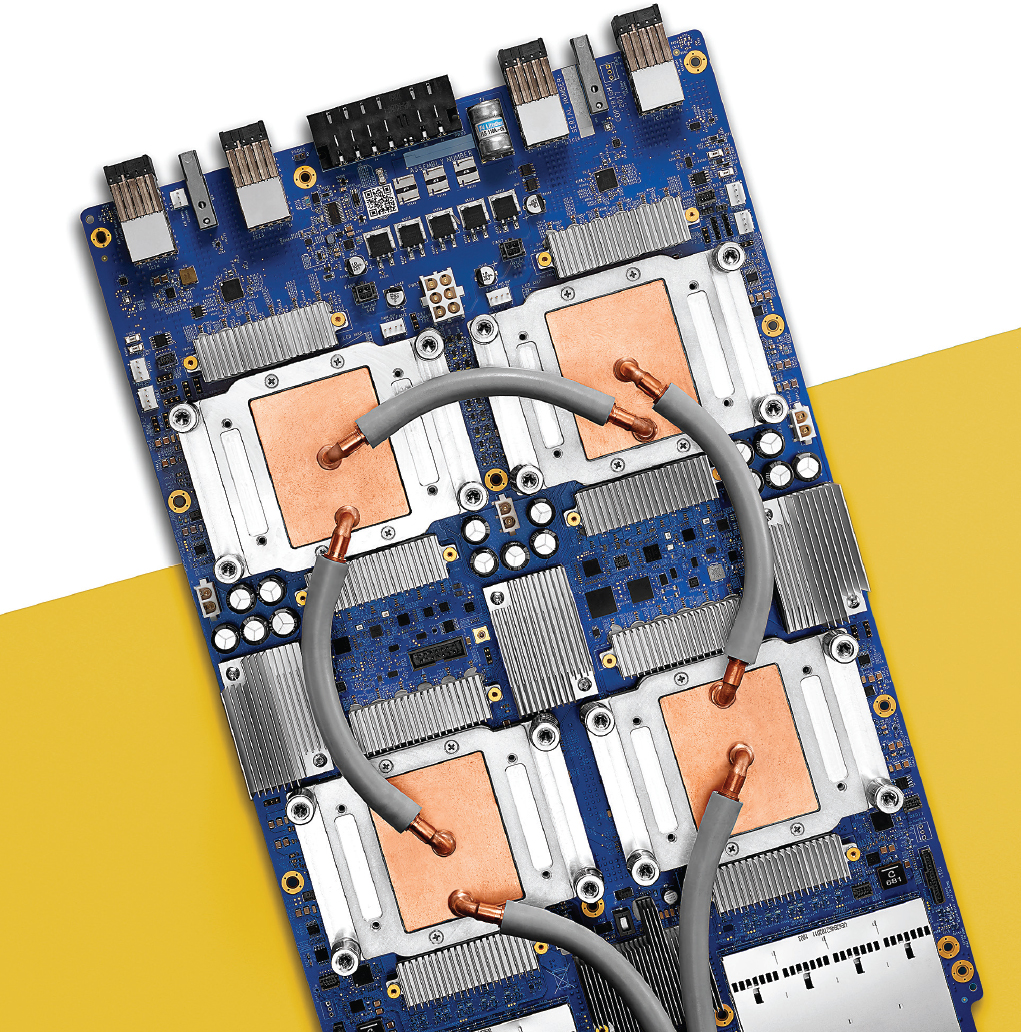
\includegraphics[scale=0.28]{google-tpu.jpeg}
	\caption{Google's TPU Chip}
	\label{fig:google-tpu}
\end{figure}

Neural network training is a fundamental process in machine learning where a model learns to make predictions by adjusting its parameters based on input data. The bulk of the mathematical operations involved in training a neural network are simply addition and multiplication instructions of floating point values. Hence, a computing device that is executing a learning algorithm for some neural network is issuing a series of floating point addition and multiplication instructions. Modern computers have specialized hardware features that allow for parallel vectorized executions of these multiply and add instructions, all in an effort to improve the training efficiency of neural networks. These hardware optimizations are particularly beneficial when dealing with larger datasets and complex network architectures.

Further specializations of hardware such as in the case of Application-Specific Integrated Circuits (ASICs) have improved upon this trend. Google's Tensor Processing Unit or TPU chip shown in Figure \ref{fig:google-tpu} is an example of such an ASIC meant to execute neural network operations, and other similar large matrix operations with great efficiency.

Most of the existing embedded hardware are not especially designed for machine learning or neural network acceleration like the ASICs. Hence, it becomes important to understand the difficulties in moving the training of a neural network to the embedded devices and the capabilities of modern software systems to complete these implementations efficiently \cite{zhu2023ondevice}. On-Device training strategies also allow for the possibility of reducing the movement of data from embedded devices to achieve learning.

\section{Federated Learning of Neural Networks}

The conventional approach to developing neural network applications on embedded devices presents a challenge due to the substantial network bandwidth consumed by continuously transmitting sensor data to a central data repository. The data from different devices are combined to form the dataset that will be used to further train the model. This data aggregation process, essential for building training datasets, exposes devices to security risks, potentially compromising sensitive behavioural information. A simplified diagram denoting the traditional model is presented in Figure \ref{fig:nn-traditional}.

\begin{figure}[h]
	\centering
	\begin{tikzpicture}
		\node (ecu) at (0,0) {
\includegraphics[scale=2]{truck.png}};
		\node at (ecu.south) {ECU};
		\node (cloud) at (3.5, 2) {
\includegraphics[scale=2]{db.png}};
		\node at (cloud.north) {Data lake};
		\node (server) at (7, 0) {
\includegraphics[scale=2]{server.png}};
		\node at (server.south) {Server};
		\draw[-{Latex}, very thick, orange!90] ([xshift=14pt]server.north east) arc (355:0:0.25);

		\draw[->,thick] (ecu) -- (cloud);
		\draw[->,thick] (cloud) -- (server);
		\draw[->,thick] (server) -- (ecu);
	\end{tikzpicture}
	\caption{Traditional neural network application architecture. Orange indicates neural network training}
	\label{fig:nn-traditional}
\end{figure}

One way to address this problem is to rely on alternative mechanisms to perform the continual training of the model in a decentralized manner. Federated learning is a technique of training machine learning models in such a distributed way, where each client device uses its own data set to train a local model. After this local training session, the new model may be sent to a central server which will combine the different models to form a new global model. This may be then sent to the client devices for performing inference. There are several algorithmic strategies to choose from to combine the local training sessions based on the differences in the data set on the embedded devices.

Training on the device optimizes bandwidth usage and minimizes latency. Instead of sending massive volumes of data over the network, only model updates which are typically much smaller are exchanged between the device and the central server. This not only conserves network resources but also accelerates the learning process, as computations occur on the device itself without waiting for data transfers. A simplified diagram representing federated learning is presented in Figure \ref{fig:nn-federated}.

Federated learning allows for joint training of vast amounts of data without exchanging that data. Another aspect to consider is how the locally trained models are sent back to a central server for combining with other such models. Some form of gradient compressions strategies may be required to ensure that the model updates do not leak information about the data on board the embedded devices.

\begin{figure}[h]
	\centering
	\begin{tikzpicture}[rounded corners, opacity=0.87]

		\readlist\Trucks {1,2,3,4}
		\foreachitem \x \in \Trucks
		{
			\node (ecu \x) at ({0 + 2.5 * (\x-1)}, 0) {
\includegraphics[scale=2]{truck.png}};
		}

		\node[inner xsep=21pt] (server) at (3.5, 2) {
\includegraphics[scale=1.8]{server.png}};
		\draw[-{Latex}, very thick, orange!90] ([yshift=-7pt]server.north east) arc (355:0:0.25);

		\foreachitem \x \in \Trucks
		{
			\draw[<->,thick] (ecu \x.north) -- (server);
			\draw[-{Latex}, very thick, orange!50] ([yshift=-7pt]ecu \x.north east) arc (355:0:0.25);
		}

	\end{tikzpicture}
	\caption{Federated Learning application architecture}
	\label{fig:nn-federated}
\end{figure}



Federated learning implementations can thus differ based on how the distributed training takes place, the algorithm to combine different locally trained models, and other strategies used in completing the development loop. In the LOBSTR \cite{lobstr} and FAMOUS \cite{famous} projects Scania has developed statistical models and neural network models for anomaly detection using a federated learning approach. The statistical models are lightweight and can easily be trained with limited computational resources.


% This thesis focuses on repurposing existing hardware (ECU) to machine learning edge devices that are tailored to train neural network in the most efficient possible way. We try to reverse engineer the old communicator model to build a custom Yocto Project tailored for ML. As alternative test ECU we use an evaluation board that has similar specifications as the communicator to benchmark and experiment different neural network implementations and evaluate.


% ============================================
%        Theory
% ============================================

\chapter{Theory}

The first section in this chapter lays out an overview of the training process of neural networks. The following section introduces some terminology associated with software development for embedded devices, contextualized in Embedded Linux.

\section{Neural Networks}

A neural network consists of a collection nodes called \textit{neurons} that are arranged into several layers with connecting edges that go between the layers. A connecting edge between two neurons describe an operation with the first neuron producing an output that is then consumed as input by the second neuron. The first layer and final layer are special and are called \textit{input layer} and \textit{output layer} respectively. There maybe zero or more layers that lie between them called \textit{hidden layers}.

\begin{center}
	\begin{tikzpicture}[x=2.4cm,y=1.2cm]
		\readlist\Shape{4,3,2}
		\readlist\Type{1,2,3}
		\readlist\Label{x,h^{(\prev)},y}

		\def\yshift{0.45}

		\foreachitem \nodes \in \Shape{
			\def\lay{\nodescnt}
			\pgfmathsetmacro\prev{int(\nodescnt-1)}

			\foreach \i [evaluate={
				\c=int(\i==\nodes);
				\y=\nodes/2-\i-\c*\yshift;
				\x=\lay;
				\n=\Type[\lay];
				}] in {1,...,\nodes} {

				\node[node \n] (nodes\lay-\i) at (\x,\y) {$\Label[\lay]$};

			\ifnum\lay>1
				\foreach \j in {1,...,\Shape[\prev]}{
				\draw[connect] (nodes\prev-\j) -- (nodes\lay-\i);
				}
			\fi
			}
			\path (nodes\lay-\nodes) --++ (0,1+\yshift) node[midway,scale=1.5] {$\vdots$};
		}
	\end{tikzpicture}
\end{center}

The connecting edges between the neurons are weighted and additionally a neuron may carry a weight of its own called \textit{bias}. The neurons may have several incoming edges, except for the neurons in the input layer, and several outgoing edges, except for the neurons in the output layer. Each neuron in the network describes a computation in at least two steps, (1) multiply input data with corresponding edge weight and take their sum along with the bias value, (2) transform the value calculated earlier using an activation function.

An activation function $\sigma$ is said to determine the activation of the neuron which can be thought of as the output that the neuron generates. There are several kinds of activation functions that are used in neural networks such as the sigmoid, ReLU, tanh, etc.

Combining these operations the neuron $y_k$ has the output

\begin{equation}
	y_k = \sigma \left( \sum_{j=0}^m w_{kj} x_j \right)
\end{equation}

Where $y_k$ is the $k^{th}$ neuron in a layer with input values $x_0$ through $x_m$ with corresponding weights $w_{k0}$ through $w_{km}$. The first input $x_0$ is usually set to $0$ and hence the corresponding weight $w_{k0}$ stands in for the bias $b_k$ of the neuron. The complete neural network matrix multiplication pass from input to output is called the \textit{feedforward}.

Neural networks can be constructed in a variety of ways with the choice for how many layers to use, the number of neurons in the layers, the connections between the layers, all of which can generate different topologies. The neural network model can approximate a real world system by modelling that system as function that takes in some input and then generating an output. The neural network can approximate this function better by changing the connections between neurons, dropping and or adding neurons, varying the weights encoded in the connections, or by varying the biases within the neurons.

Once a neural network completes a training on a training set, it can then be used to look at data points that it has not seen previously. The neural network can be made to perform the feedforward calculations to produce some prediction or output and this step is said to be a neural network \textit{inference}.

\subsection{Neural Network Training}

One of the most interesting characteristics of a neural network is its capacity to form probability weighted associations between a set of inputs and their corresponding outputs. The process of forming this association is called \textit{training} the neural network, the set of input patterns used for this purpose is called a \textit{training set}, and the algorithm by which the network is trained is called the \textit{learning algorithm}. After sufficient training, the network can also produce correct outputs to unseen inputs of the same kind.

In the domain of neural network training, \textit{Stochastic Gradient Descent (SGD)} is the cornerstone learning algorithm. This technique enables neural networks to learn from data, adjust their parameters, and improve their performance over time. To provide a more insightful analogy, envision an expansive and undulating landscape representing the manifold possibilities of values a neural network model can have. This terrain serves as the state space for the learning algorithm. The aim of the learning algorithm is to locate the lowest point in this space. This point corresponds to the lowest error for the neural network model.

While the complete view of the terrain will be hidden, the direction of the steepest descent can be understood as the path of with the least resistance. Similarly, the \textit{gradient descent} approach guides the learning algorithm by providing the values to adjust the network. In essence, SGD exploits this concept to iteratively adjust model parameters, descending towards optimal configurations, and thus facilitating the model's refinement and improved predictive capabilities over successive iterations.

The goal of the SGD algorithm is to minimize a \textit{loss function}, which quantifies the discrepancy between the predicted outputs of the network and the actual target values. The gradient of this loss function provides the direction of the steepest ascent, and by moving in the opposite direction, we can descend toward the minimum. Mathematically, given a loss function $\mathcal{L}$ and parameters $w$, the gradient descent update step can be expressed as:

\begin{equation}
    w_{new} = \theta - \eta \cdot \nabla \mathcal{L}(w)
\end{equation}

Here, $\nabla \mathcal{L}(w)$ is the gradient of the loss with respect to the current parameters $w$, and $\eta$ is the \textit{learning rate}, a hyperparameter that controls the step size. The learning rate governs the trade-off between \textit{convergence speed} and \textit{stability}. Convergence speed refers to how quickly a learning algorithm approaches its optimal solution while stability refers to the ability of the learning algorithm to consistently produce reliable and predictable results.

Calculating the gradient over the entire dataset for each update can be computationally expensive. SGD addresses this challenge by introducing randomness and \textit{mini-batch sampling}. Instead of computing the gradient using all data points, SGD randomly selects a subset of the data called the \textit{mini-batch} for each update. This not only speeds up the computation but also adds a form of noise that can help the learning algorithm escape local minima.

\begin{equation}
    w_{new} = w - \eta \cdot \nabla \mathcal{L}(w; \textit{mini-batch})
\end{equation}

Another important improvement to how the learning algorithm works is in techniques used to calculate the gradient weights. The \textit{backpropagation} algorithm is a critical mechanism used to update the weights of a neural network during the training process. It involves computing the gradients of the network's loss function with respect to its parameters by traversing the network in reverse order, from output to input layers. These gradients quantify the impact of each parameter on the overall error, enabling the network to adjust its parameters in a direction that minimizes the error. Backpropagation in SGD enhances the convergence of the optimization process by iteratively adjusting weights based on the computed gradients and a small learning rate, ultimately guiding the network towards better performance and improved ability to generalize to unseen data.

\section{Embedded Linux}

As presented in the previous chapter, the development, deployment, and maintenance of Embedded Linux distributions and their user mode applications are usually managed using capable build systems. Configuring these systems requires understanding concepts such as bootloaders, device tree layouts, flash memory, cross compiling toolchains, board support package, etc. with the later two having already been introduced in the preceding chapter.

Porting an Embedded Linux distribution on some embedded hardware completes successfully when the processor on the board is able to run the Linux operating system. Depending on hardware several paths may be taken by the processor to reach this stage after powering on. This process of starting the computer is called \textit{booting} and the sequence of stages the board goes through is called \textit{boot sequence}. Embedded devices are greatly varied and hence there is great variance in how boot sequence take place. The next part of this section introduces yet more concepts and terminology around the boot sequence for a commonly used embedded board running an Embedded Linux.

\subsection{An Overview of the Standard Boot Sequence}

After power up, the processor requires initialization of its constituent hardware components. The processors usually found in ECUs will have this function performed by \textit{firmware} placed in a special purpose memory called \textit{boot ROM}. Firmware is software that provides low level control of a devices specific hardware that is placed on embedded hardware by the silicon vendor or the system maker. The boot ROM, as the name suggests, is a type of read-only memory that is usually placed close to the processing unit. After powering on, the processor is said to come out of reset. The processor is designed to look up the memory mapped to the boot ROM after reset. The boot ROM code then starts executing on the processor and starts initializing peripheral devices, hardware busses, CPU registers, etc. After initializing the hardware, the boot ROM code is responsible for locating and loading a bootloader program. At this point the boot ROM may also perform additional verification procedures such as \textit{checksum} validation. Checksum is a small block of data derived from another usually larger block of data that is used for the purpose of detecting errors or performing data integrity checks. The boot ROM may have some way of checking the data present inside a flash memory and computing a checksum calculation to verify based on some notion of data integrity. This location is usually on some external memory to the processor such as an \textit{embedded MultiMediaCard} (eMMC). eMMC is one among several memory card standards for solid state memory storage.

Bootloader programs are responsible for continuing the boot process and may have multiple stages with one stage loading another. The first stage of booting may deal primarily with configuring the memory controller, and the main memory such as a \textit{synchronous dynamic RAM} (SDRAM). The second stage of the boot process may then deal with identifying and preparing an operating system to complete the boot. The second stage may also have to configure additional peripheral devices, perhaps even provide an interface to select between different versions of operating systems available on across the peripheral memory devices. U-Boot is the most commonly used open source bootloader for embedded devices. U-Boot will normally be stored in some storage medium that will be accessible by the boot ROM code, usually some flash memory. Flash memory is a kind of non-volatile memory that can be electrically erased and reprogrammed and is commonly used for storing data and firmware. Flash memory comes in two kinds, NOR flash and NAND flash which have different performance characteristics and usage scenarios. Different flash memory standards rely on either a NOR flash or NAND flash based scheme, for e.g. the eMMC standard uses NAND flash.

U-Boot may also be divided into multiple stages, as described previously, on different flash memory. One such multistage division for U-Boot is into the \textit{Secondary Program Loader} (SPL) and a more fully featured U-Boot. SPL could then provide the first stage of the boot procedure and hand over control to the more fully featured U-Boot as the second stage. After getting control of the processor, U-Boot then has to take care of initializing the memory system, finding then loading the Linux kernel into an appropriate location in memory, generate boot parameters for the kernel, and copy other required data for the kernel. The kernel is also commonly stored on a flash memory on board. One of the configuration data that U-Boot has to pass to the kernel is the device tree, which is a data structure describing the hardware layout. Device trees were adopted in Linux and the embedded industry in general to allow mainline Linux and U-Boot to use the device tree to run on a particular board configuration, and to dissuade the creation of U-Boot and Linux forks to target marginally different boards \cite{device-tree}.

U-Boot implements a subset of the Unified Extensible Firmware Interface (UEFI) specification outlining the architecture of the device firmware used to boot and its interaction interface with the operating system. The full feature set of U-Boot includes an UEFI compatible boot manager utility, a device management utility, explicit memory handling to allow data copying and kernel execution, and a command line interface (CLI) to provide access to these features.

U-Boot starts by locating the kernel to be loaded. The linux kernel is usually stored in some compressed form and the first step U-Boot takes is to decompress that kernel from flash memory, onto the main memory. After U-Boot completes its tasks, it gives up control over the processor to the kernel. The control ends up with the \texttt{start\_kernel} method in the kernel code, which is an architecture independent starting point for the rest of the Linux kernel boot process. The kernel proceeds with yet more configuration steps such as configuring the memory, processor, peripherals, cache, and other hardware devices.

The \textit{process} abstraction in Linux refers to the concept of treating running programs as independent and isolated entities that operate concurrently within the same system. Each process represents the execution of a program and is allocated its own view of memory and system resources like the CPU time and I/O operations. Processes in Linux are managed by the \textit{scheduler}. After configuring the processor, memory, and other peripherals, the kernel proceeds to complete its start up by setting up kernel data structures in memory, initializing the scheduler, setting up and allocating \textit{pages}, etc. A memory page is a fixed size block of data used in virtual memory systems serving as a unit for memory allocation, management, and data exchange between physical RAM and secondary storage devices. The virtual memory system is a memory management technique used by modern operating systems to provide an abstraction of a larger and more flexible memory space to applications than is physically available in the computer's physical RAM. It allows programs to use memory addresses that are independent of the actual physical addresses of the underlying hardware. This enables efficient memory usage, process isolation, and the ability to run larger programs than the available physical RAM would allow.

\begin{figure}[h]
	\centering
	\begin{tikzpicture}
		\node [box] (rom) {Boot ROM};
		\node [box, right=of rom] (uboot) {UBoot};
		\node [box, right=of uboot] (kernel) {Kernel};
		\node [box, right=of kernel] (init) {Init};

		\draw [next] (rom) -- (uboot);
		\draw [next] (uboot) -- (kernel);
		\draw [next] (kernel) -- (init);
	\end{tikzpicture}
\end{figure}

The kernel completes the start-up after initializing the root filesystem and spawning the \texttt{init} process, which is the first process to that starts after booting completes. The \texttt{init} process is responsible for bringing up several user level programs and system services. Processes are created through a mechanism called "forking," where an existing process (parent) generates a copy (child) with its own memory and execution state. The \texttt{init} process in this manner acts as the ancestor process for all other processes. Once the kernel has successfully initiated the init process, the user space environment is said to be instantiated and the higher-level processes and applications take over. At this point, the system becomes operational and ready for user interaction and application execution.
